\documentclass[12pt]{article}
\usepackage[a4paper, margin=2cm]{geometry}
\usepackage[english]{babel} % To obtain English text with the blindtext package
\usepackage{blindtext}
\usepackage{graphicx} % Required for inserting images
\usepackage{array, multirow} % For extra column formatting
\usepackage{amsmath, amssymb, cancel} %for equation environment
\usepackage{float}
\usepackage{parskip} % For gaps between para
\usepackage{setspace}
\usepackage{pdfpages}
\usepackage{abstract}
\usepackage[export]{adjustbox}
\usepackage{emptypage}
\usepackage{tocloft}
\usepackage[nottoc]{tocbibind}
\usepackage{hyperref, url}
\usepackage[table]{xcolor}
\usepackage{minted}
    \usemintedstyle{monokai}
\usepackage{caption,subcaption}
    \captionsetup{font=footnotesize,labelfont=bf,textfont=it}
\usepackage{tcolorbox}
    \newtcolorbox{mintedbox}{
        colback=backcolour,
        boxrule=0pt,
        sharp corners,
        width=\linewidth,
        left=0pt, right=0pt,
        top=3pt, bottom=3pt
    }
\usepackage{fancyhdr,titlesec,bookmark,threeparttable,wrapfig}
\usepackage[numbers]{natbib}
\usepackage[export]{adjustbox}
\usepackage[outercaption]{sidecap}

\setlength{\headheight}{15pt}  % Ensure enough space for the header
\addtolength{\topmargin}{-2pt} % Adjust to prevent overflow

\pagestyle{fancy}
\fancyhf{} % Clear defaults
\renewcommand{\sectionmark}[1]{\markright{#1}} % Stores section title
\fancyhead[L]{\rightmark} % Left header
\fancyhead[R]{\textbf{Ariel}}
\fancyfoot[C]{\thepage}
\renewcommand{\headrulewidth}{0.4pt}  % Default thin line

\pagenumbering{arabic}

\cftsetindents{section}{0em}{2em}
\cftsetindents{subsection}{0em}{2em}

\renewcommand\cfttoctitlefont{\hfill\Large\bfseries}
\renewcommand\cftaftertoctitle{\hfill\mbox{}}

\graphicspath{ {./images/} }

\definecolor{blurple}{HTML}{5865F2}
\definecolor{backcolour}{HTML}{272823}

\hypersetup{
    colorlinks=true,
    linkcolor=black,
    urlcolor=black,
    citecolor=blurple,
}

\urlstyle{same}

\renewcommand{\arraystretch}{1.3}

\setcounter{secnumdepth}{5}
\setcounter{tocdepth}{5}
\newcommand\simpleparagraph[1]{%
  \stepcounter{paragraph}\paragraph*{\theparagraph\quad{}#1}}

\hbadness=11000

%%%%%%%%%%%%%%%%%%%%%%%%%%%%%%%%%%%


\title{PHYC20040 Ariel Mission}
\author{Joana Adao}
\date{\today}

\begin{document}

\begin{titlepage}
    \begin{figure}[H]
        
\includegraphics[width=.8\textwidth]{UCDLogo.png}
    \end{figure}

    \begin{center}
        \vspace{4cm}

        {\LARGE \bfseries Ariel Mission Research Report}\\
        \vspace{0.5cm}
        {\Large Atmospheric Remote-Sensing Infrared Exoplanet Large-Survey}\\
        \vspace{2cm}
        {\Large \textbf{PHYC20040 Exploring the Solar System}}\\
        
        \vspace{1cm}
    

    \vspace{2cm}
    
    {\large \textbf{by}}\\
    \vspace{.5cm}
    {\normalsize Joana Carranço Cabral Adão, Kyla Boyle, Ewan Finlayson, Ananya Laxmeshwar, Isha Mathew, Matilda Onnebrink, Brian Woods}\\

    \end{center}
    
   \clearpage

\end{titlepage}

\tableofcontents
\thispagestyle{empty}

\newpage

%%%%%%%%%%%%%%%%%%%%%%%%%%%%%%%%%%%

\thispagestyle{empty}

\begin{center}
    {\Large \textbf{Ariel Mission Research Report}}\\

    \vspace{.4cm}
    {\large Atmospheric Remote-Sensing Infrared Exoplanet Large-Survey}\\

    \vspace{1cm}
    \begin{minipage}{.8\textwidth}
        \centering
        \small
        \textbf{Joana Carranço Cabral Adão, Kyla Boyle, Ewan Finlayson, Ananya Laxmeshwar, Isha Mathew, Matilda Onnebrink, Brian Woods}
    \end{minipage}
    \vspace{2.3cm}

    \begin{abstract}
    \addtocontents{toc}{\protect\contentsline{section}{\textbf{Abstract}}{\hfill}{}} 

    Ariel, the Atmospheric Remote-sensing Infrared Exoplanet Large-survey, is a mission that's part of ESA's Cosmic Vision program due to launch in 2029 and aimed at studying the chemical composition and thermal structures of exoplanet atmospheres.
    Using infrared spectroscopy, Ariel is set to observe thousands exoplanets with focus on those hotter than 600 K in close orbits around their stars. By analysing their atmospheric makeup, including key chemical compositions,
    Ariel will help scientists better understand the diversity of exoplanet environments, providing crucial insights into planetary formation and evolution.
    Ariel will be the first mission dedicated to this task, paving the way for future missions that will expand our knowledge of exoplanets, including potentially habitable worlds.

    \end{abstract}
\end{center}

\newpage

%%%%%%%%%%%%%%%%%%%%%%%%%%%%%%%%%%%

\setcounter{page}{1}
\section{Introduction} \label{sec:1}

Over the past two decades, thousands of exoplanets have been discovered by various international missions, including potentially habitable planets around nearby stars.
Many more are expected to be discovered by ground and space-based telescopes in the near future \cite{madhusudhan2019exoplanetary}.
These discoveries have led to rapid progress in the field of planetary science.

NASA's Kepler mission and the subsequent K2 mission alone found over 3000 exoplanets in habitable zones with hundreds more yet to be confirmed. The Transiting Exoplanet Survey Satellite (TESS)
found over 600 exoplanets and thousands more to be confirmed \cite{exoplanet_and_candidate_statitics_2025}. These missions, however, are primarily focused on detecting planetary transits and measuring the orbital parameters of such exoplanets \cite{zingales2018ariel}.

The next significant research opportunity for the field lies in the spectroscopic observation of exoplanets' atmospheres \cite{madhusudhan2019exoplanetary}.
Studying exoplanetary atmospheres is key to understanding planetary formation and evolution \cite{zingales2018ariel}.

It can now be said that "we have entered the era of comparative exoplanetology" \cite[p. 617]{madhusudhan2019exoplanetary}.
Currently, only some exoplanetary atmospheres have been studied, and they have revealed new insights into the diversity of their chemical compositions and atmospheric processes \cite{madhusudhan2019exoplanetary}.
More are expected to be studied by the James Webb Space Telescope (JWST) and the ground-based Extremely Large Telescope (ELT) \cite{beichman2014observations}.

The European Space Agency's new Atmospheric Remote-sensing Infrared Exoplanet Large-survey (Ariel) mission, expected to launch in 2029, will be the first to study a statistically significant sample of over
500 candidates for exoplanetary atmospheres \cite{zingales2018ariel}.
The atmospheric data collected by Ariel is therefore expected to make a large contribution to the field of planetary science.

The Ariel telescope will be used to study molecular composition, cloud coverage, and thermal structures of exoplanet atmospheres using transit spectroscopy. The results will allow for a re-examination of 
current models of planet formation by linking the collected atmospheric data to the stellar properties of the planets' host stars, and improve our understanding of atmospheric evolution across planetary systems \cite{edwards2019updated}.

This report provides an overview of the Ariel mission, outlining its scientific objectives, expected findings and challenges, and scientific istrumentation. It gives an in-depth explanation of the motivation behind the mission and its importance and validity
in a competitive environment, where limited funding and resources dictate mission selection.

\subsection{Motivation for Ariel}



\subsubsection{Importance of Studying Exoplanets}


\newpage

\section{Scientific Objectives}

\subsection{Past Exoplanet Characterisation Efforts}



\subsection{Criteria for Exoplanet Selection}

In order for the selected sample of observed exoplanets to be statistically significant and representative, both the number of observed planets and the sample must be diverse \cite{zingales2018ariel}.
The planets must therefore be selected in accordance to various criteria; the sample must contain both gaseous and rocky planets across a range of temperatures, and the host stars must also be of
different spectral types and metallicity. A correspondingly large number of planets covering the widest possible spectrum can be sourced and selected from exoplanets discovered by previous missions, such as
the Kepler Space Mission \cite{zingales2018ariel} and the Transiting Exoplanet Survey Satellite (TESS) \cite{arielTESScandidates}.

The Ariel mission will focus primarily on planets with an orbital period that's less than 50 days, typically corresponding to warmer planets. 

\subsection{Ariel Tier List System for Observational Prioritisation}

To maximise the science return of the Ariel mission, a three-tiered system has been devised where the three different samples are observed at optimised spectral resolutions, wavelength intervals,
and SNR \cite{salvignol2024ariel}. An additional fourth tier has been planned for additional science time to observe the pahse curves of Tier 3 planets \cite{arielstudyreport} (see Table \ref{tab:1}, Table \ref{tab:2}).

\begin{table}[H]
    \caption{Table of the Ariel tiers presented, with percentage of dedicated mission lifetime and requirements for each tier shown \protect\cite{arielstudyreport,salvignol2024ariel}.}
    \centering
    \label{tab:1}
    \resizebox{\textwidth}{!}{        
        \begin{threeparttable}
            \renewcommand{\arraystretch}{1.55}
            \begin{tabular}{|l@{\hskip 15pt}|l|}
            \hline
            Survey ($\sim$30\%)\protect\tnote{**} &
            \begin{tabular}[c]{@{}l@{}}Low spectral resolution observations (R $\geq$ 10 across all channels) of a large sample\\ of planets in the VIS-IR, with SNR $\geq$ 7\end{tabular} \\ \hline
            Deep ($\sim$60\%)\protect\tnote{**} &
            \begin{tabular}[c]{@{}l@{}}Intermediate spectral resolution observations (R $>$ 50 in AIRS channel 0 and R $>$ 15 \\ in AIRS channel 1) of a sub-sample in the VIS-IR\end{tabular} \\ \hline
            Benchmark ($\sim$6\%)\protect\tnote{**}    & Very best planets, re-observed multiple times with all techniques; full spectral resolution \\ \hline
            Phase Curves ($\sim$4\%)\protect\tnote{**} & Multiple-band photometry/spectroscopy with SNR $\geq$ 4; spatial variability                     \\ \hline
            \end{tabular}%
            \begin{tablenotes}
                \footnotesize
                \item[**] \textit{\% correspond to mission lifetime spent at each tier}
            \end{tablenotes}
        \end{threeparttable}
    }
\end{table}

\begin{table}[H]
    \caption{The total science time is $\sim$24 800 hr over the primary 4 year mission lifetime. Table of mission time required to achieve different observation goals. Note that for some bright targets (e.g. HD 209458b) Tier 2 or Tier 3 
    resolutions would be reached in a single observation \protect\cite{arielstudyreport}.}
    \centering
    \label{tab:2}
    \resizebox{.8\textwidth}{!}{%
        \begin{tabular}{lcc}
        \multicolumn{3}{c}{Mission Time Required to Achieve Different Observation Goals}                                                                       \\ \hline
        \textbf{Number of Planets} &
        \textbf{Observation Requirement} &
        \textbf{Required Science Time (hr)} \\ \hline
        1000 & Achieve Tier 1 resolutions                                                               & $\sim$10 600 \\ \hline
        \begin{tabular}[c]{@{}l@{}}400\\ \\ 500\\ 600\end{tabular} &
        \begin{tabular}[c]{@{}c@{}}Increase resolution from Tier 1\\ to Tier 2\end{tabular} &
        \begin{tabular}[c]{@{}c@{}}$\sim$3100\\ \\ $\sim$6000\\ $\sim$10 500\end{tabular} \\ \hline
        \begin{tabular}[c]{@{}l@{}}200\\ \\ 300\\ 400\end{tabular} &
        \begin{tabular}[c]{@{}c@{}}Achieve Tier 1 resolutions in the\\ second method\end{tabular} &
        \begin{tabular}[c]{@{}c@{}}$\sim$1400\\ \\ $\sim$2500\\ $\sim$4200\end{tabular} \\ \hline
        50   & \begin{tabular}[c]{@{}c@{}}Tier 3 (five repeated observations\\ per planet)\end{tabular} & $\sim$1700   \\ \hline
        ...  & Tier 4 (additional science time)                                                         & $\sim$2300   \\ \hline
        \end{tabular}%
    }
\end{table}

The orbit and attitude limits of the spacecraft must also be considered for measurements during scheduling in order to maximise the science time. Figure \ref{fig:1} illustrates the distribution of targets in right ascension and declination (equatorial) coordinates for the fraction of the year
that each region of the sky is visible within Ariel's assumed proposed orbit at the Sun-Earth Lagrangian point L2. Any direction is observable for at least $\sim$30\% of the year \cite{zingales2018ariel,morales2022ariel}.

\begin{figure}[H]
    \centering
    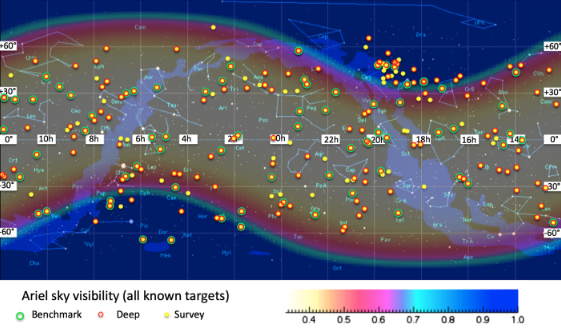
\includegraphics[width=.9\textwidth]{ariel target map.png}
    \caption{A plot illustrating the fraction of the year for which a given location in the sky (in equatorial coordinates) is visible to Ariel, as seen from a representative operational
    orbit of Ariel at L2. \textbf{Yellow} dots: planets observed in Tier 1. \textbf{Red} dots: planets observed in Tier 2. \textbf{Green} dots: planets observed in Tier 3. \protect\cite{zingales2018ariel} The background colour levels represent the fraction of the year for which
    region of the sky is visible for Ariel \cite{morales2022ariel}.}
    \label{fig:1}
\end{figure}

\subsubsection{Survey (Tier 1)}

Tier 1 observations will help refine orbital and planetary parameters that can then be used to limit or completely remove degeneracies in the interpretation of mass-radius diagrams.
Most giant planets and Neptunes fulfil the Tier 1 criteria set for the science objectives in 1 transit/eclipse, while the smaller planets would require upwards fo 6 events (see Figure \ref{fig:3}) \cite{zingales2018ariel}.
Additionally, it will be possible to generate colour-colour and colour-magnitude diagrams, which might lead to the same developments in understanding as the H-R diagram did \cite{edwards2019updated,salvignol2024ariel}.

\begin{figure}[b]
    \centering
    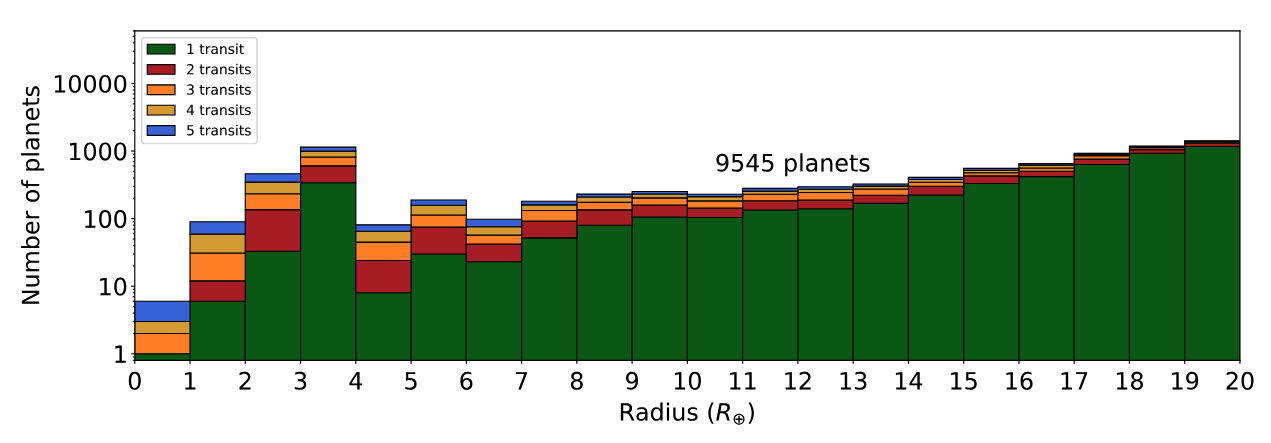
\includegraphics[width=.9\textwidth]{tier 1 transit graph.png}
    \caption{Complete set of Tier 1 planets from the Ariel mission reference population. The final list of Tier 1 planets will include an optimal sub-sample. Different colours indicate the number of transits/eclipses needed to reach
    Tier 1 performances. The planets shown here can achieve the Tier 1 requirements combining the signal of $\leq$ 5 transits/eclipses \protect\cite{zingales2018ariel}.}
    \label{fig:3}
\end{figure}

Tier 1 observations will answer the following questions:

\textbf{"What fraction of planets are covered by clouds?"}\\
This method of observation between planets with clear atmospheres and those denser cloud cover, as this obscures molecular absorption features typically present in spectra.
Extremely cloudy planets can be identified from low-resolution across a broad wavelegnth range. This assessment allows scientists to determine whether a planet should continue with higher-resolution spectral classification
(i.e., be included in the Tier 2 sample) or not \cite{salvignol2024ariel}.\\

\textbf{"What fraction of small planets still have hydrogen and helium retained from the protoplanetary disc?"}\\
This question is essential to understand the formation and evolution of super-Earths. Primordial (or primary) atmospheres are expected to be consisted of mainly hydrogen and helium,
reflecting the gaseous composition of the protoplanetary nebula. If an atmosphere is made up of heavier metals, it likely indicates that the atmosphere has evolved and thus resulting in a secondary atmosphere.
The easiest way to differentiate between primary (hydrogen-rich) and secondary (metal-rich) atmospheres is through transmission spectroscopy as the main atmospheric component directly affects the atmospheric scale height \cite{salvignol2024ariel}. \\

\textbf{"What is the bulk composition of the terrestrial exoplanets?"}\\
Planetary density provides insight into the composition of a planet's interior, but this measurement alone may lead to non-unique interpretations. Analysing the composition of the upper atmosphere in transiting planets will help reveal the degree 
of composition separation between the planet's atmosphere and interior. This approach reduces uncertainties in the presence and mass of the atmosphere, therefore resolving potential doubtfulnes in understanding the planet's overall makeup \cite{salvignol2024ariel}. \\

\textbf{"What is the energy balance of the planet?"}\\
Through analysis of eclipse measurements in optical and infrared wavelengths scientists can determing the overall temperature and albedo (the fraction of diffracted sunlight) of the planet. These measurements
help estimate the planetary energy balance and whether the planet has an internal heat source or not \cite{salvignol2024ariel}.

Ariel's Tier 1 survey mode will allow for fast and comprehensive initial assessments of planets, which allows for informed decisions when deciding what planets to further focus on during Tier 2 and Tier 3 observations \cite{salvignol2024ariel}.
Observing Figure \ref{fig:2}, illustrating the distribution of potential Tier 1 targets for the Ariel mission as functions of planetary radius and temperature, it can be seen that over 500 currently known planets already comply with the requirements for Tier 1 observations \cite{arielstudyreport,edwards2019updated}.

\begin{figure}[H]
    \centering
    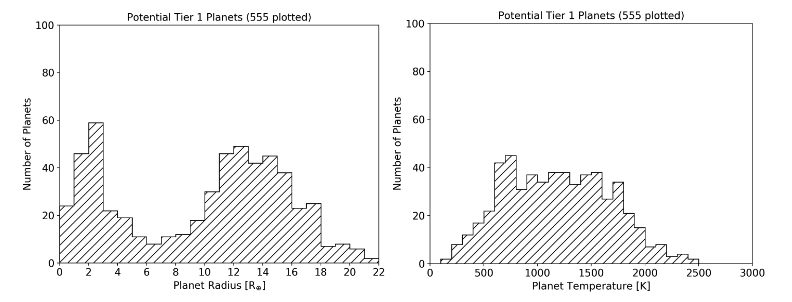
\includegraphics[width=.9\textwidth]{tier 1 radius and temp plots.png}
    \caption{Currently known Ariel planetary candidates plotted as a function of planetary radius (left) and planetary temperature (right) \protect\cite{arielstudyreport}.}
    \label{fig:2}
\end{figure}

\subsubsection{Deep (Tier 2)}

A key objective of the Ariel mission is to investigate whether a correlation exists between a planet's chemical composition and the fundamental properties such as mass, radius, and temperature. To achieve this, the Tier 2 observations will conduct high-resolution spectroscopic measurements with focus on studying both individual
exoplanets and populations. This approach allows for detailed examinations of various exoplonatery atmospheric characteristics, including \cite{salvignol2024ariel}:

\begin{itemize}
    \item[-] \textbf{Primary Atmospheric Composition in Smaller Planets:} Identifying the main gases in the atmosphere of smaller exoplanets, which is essential for characterising their atmospheric properties \cite{salvignol2024ariel}.
    \item[-] \textbf{Trace Gas Abundance:} Measuring the abundance and concentration of trace gases to determine the type of chemistry happening in the atmosphere, and whether it is in equilirbrium of non-equilibrium states \cite{salvignol2024ariel}.
    \item[-] \textbf{Atmospheric Thermal Structure:} Analysing the thermal structure, both vertically and horizontally, of the atmosphere to understand the impact on atmospheric structure and energy distribution \cite{salvignol2024ariel}.
    \item[-] \textbf{Cloud Characteristics:} Examining cloud properties, such as particle size and distribution, to understand their impact on climate and atmospheric dynamics \cite{salvignol2024ariel}.
    \item[-] \textbf{Elemental Composition in Gaseous Planets:} Investigating the elemental makeup of gaseous planets to constrain formation models and enhance the understanding of planetary evolution \cite{salvignol2024ariel}.
\end{itemize}

By integrating these measurements, the Tier 2 Deep Survey observations aim to provide a comprehensive view and understanding of atmospheric characteristics in a broad range of exoplanets, enabling comparisons across different planetary populations and contributing to the advancement of the broader goals of the Ariel mission \cite{salvignol2024ariel}.

\subsubsection{Benchmark (Tier 3)}

The Ariel Tier 3 observations are dedicated to the detailed study of atmospheric variability in a select group of exoplanets, known as benchmark planets. A portion of these planets, particularly those obiting very bright stars, will be observed multiple times over an extended period of time to gather essential data. The key objectives of these observations include \cite{salvignol2024ariel}:

\begin{itemize}
    \item[-] \textbf{Primary Knowledge of Planetary Chemistry and Dynamics:} Examining the chemical processes within exoplanet atmospheres to better understand their composition and behaviour \cite{salvignol2024ariel}.
    \item[-] \textbf{Elemental Composition Analysis:} Investigating the distribution of elements, both within the atmosphere and on the planet's surface, to gain insights into formation and evolutionary history \cite{salvignol2024ariel}.
    \item[-] \textbf{Weather Patterns and Atmospheric Variability:} tracking spatial and temporal changes in atmospheric conditions, including temperature variations, cloud coverage, and atmospheric circulation dynamics, to gain insight into the weather systems of exoplanets \cite{salvignol2024ariel}.
\end{itemize}

Benchmark planets are identified as ideal candidates for phase-curve spectroscopic measurements due to their high spectral resolution and strong signal-to-noise ratios (SNR), allowing for meaningful observations in just one or two observations.
The focus will be on "weather planets", selected for their potential to showcase significant atmospheric changes over time \cite{salvignol2024ariel}.

By conducting repeated observations, Ariel Tier 3 observations aim to capture the temporal evolution of exoplanetary atmospheres, revealing essential insights into cloud formation, atmospheric circulation, and climate dynamics on exoplanets \cite{salvignol2024ariel}.
Figure \ref{fig:4} shows a possible MRS (Mission Reference Sample) with all the three tiers discuss (Survey, Deep, Benchmark) nested together, optimised to yield maximum number of targets. 

\begin{figure}[b]
    \centering
    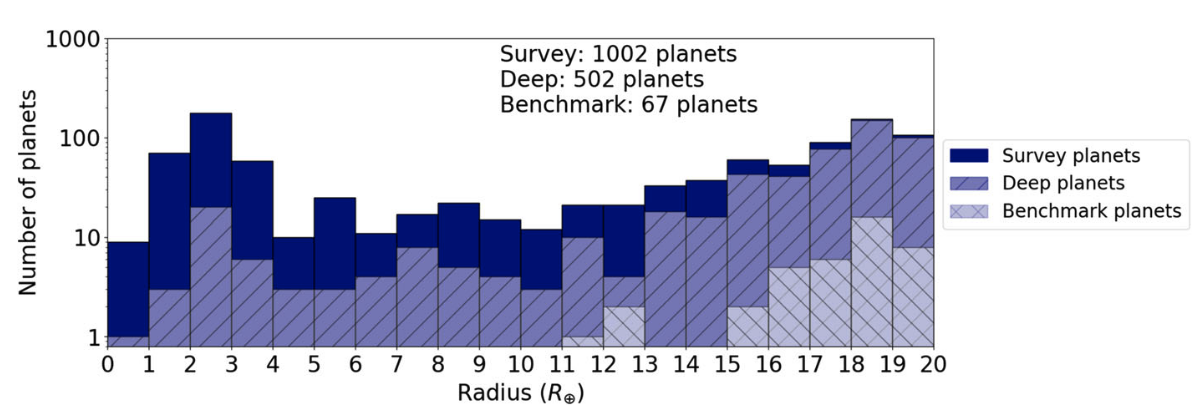
\includegraphics[width=.9\textwidth]{comparison tiers.png}
    \caption{Overview of the Ariel MRS (Mission Reference Sample), comparing the number of planets observable in the three tiers during the mission lifetime \protect\cite{zingales2018ariel}.}
    \label{fig:4}
\end{figure}

\subsubsection{Phase Curves (Tier 4)}

To gain deeper insights on targets of special interest, bespoke observations are conducted to study their spatial variability and gather detailed information on planetary chemistry and atmospheric dynamics. 
Tier 4 planets will be selected from Tier 3 Benchmark planets based on their potential to exhibit significant atmospheric variability (see Figure \ref{fig:5}) \cite{edwards2022ariel}.
A key method used in analysis is through observing planetary phase curves, which answers several fundamental questions \cite{arielstudyreport}:

\begin{itemize}
    \item[-] \textbf{Factors Influencing Atmospheric Heat Redistribution:} This investigation aims to identify how factors such as stellar irradiation, planetary radius, metallicity (the abundance of elements heavier than hydrogen and helium), and orbital eccentricity
    impact the atmospheric heat redistribution. By measuring dayside and nightside emissions, as well as phase offsets, researchers can gain details about circulation regimes, radiative timescales, wind speeds, and the role of nightside clouds \cite{arielstudyreport}.
    \item[-] \textbf{Variations in Atmospheric Composition and Thermal Structure:} This analysis focuses on how the chemical composition and thermal structure of strongly irradiated planets change from the dayside to the nightside. Atmospheric circulation is expected to smooth
    out variations, leading to chemical disequilibrium, and potential temperature fluctuations and thermal variations on the dayside \cite{arielstudyreport}.
    \item[-] \textbf{Atmospheric Composition of Low-Mass Planets:} A key objective is determining the atmospheric composition and metallicity of low-mass exoplanets. It is predicted that planets with higher atmospheric metallicity will exhibit greater heat redistribution and higher
    amplitude phase curves, allowing or independent measurements of atmospheric metallicity \cite{arielstudyreport}.
    \item[-] \textbf{Albedo of Exoplanets:} This question investigates the nature of tiny particles present in exoplanetary atmospheres, particularly condensate clouds and photochemical hazes. Measuring the planet's albedo is important for understanding its temperature balance.
    Since temperature variations can influence the albedo, understanding this relationship can provide valuable insights into exoplanet climate and atmospheric conditions \cite{arielstudyreport}.
\end{itemize}

By integrating these observations, researchers can develop a more comprehensive understanding of exoplanetary atmospheres, their dynamic, chemistry, and climate, further advancing the field of comparative planetology.

\begin{SCfigure}[50][hb]
    \centering
    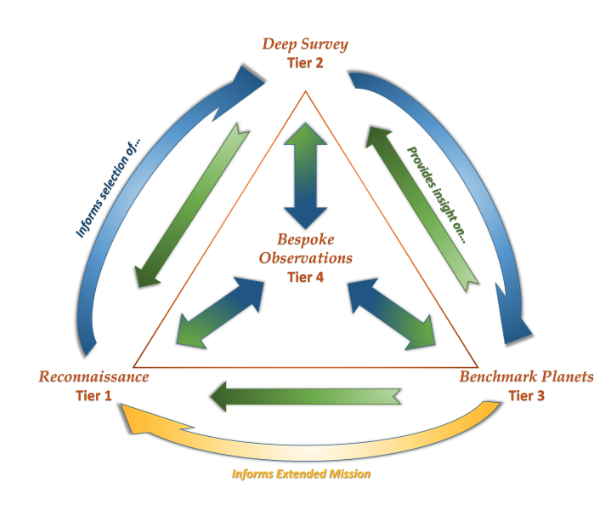
\includegraphics[width=.55\textwidth]{tiers ariel.png}
    \caption{Schematic diagram of Ariel's 4-Tier ecosystem. Tier 1 will provide the base for selecting Tier 2 planets, which in turn inform the selection of Tier 3 targets. The planets in each Tier will give us deeper insight into the nature of the planets in preceding Tiers. This interdependence among Tiers means that the
    scientific value of the data collected by Ariel will grow over time. Tier 4 observations will benefit from the insight gained by the planetary populations of the other Tiers and will in turn provide a better understanding of their atmospheric behaviour \protect\cite[p. 40]{arielstudyreport}.}
    \label{fig:5}
\end{SCfigure}

\subsection{Expected Discoveries}

\newpage

\section{Spacecraft Overview}

\subsection{General Spacecraft Design}


\subsubsection{Key Components and Subsystems}


\subsection{Service Module (SVM)}


\subsection{Payload Module (PLM)}

\newpage

\section{Payload Instrumentation and Technology}

\subsection{Optical and Spectroscopic Instruments}


\subsection{Calibration and Performance}


\subsection{Data Transmission and Storage}

\newpage

\section{Mission Operations and Timeline}

\subsection{Launch and Deployment}


\subsection{Orbital Parameters}


\subsection{Operational Phases}


\newpage

\section{Conclusion}

\newpage

%%%%%%%%%%%%%%%%%%%%%%%%%%%%%%%%%%%

\bibliographystyle{IEEEtran}
\bibliography{References} \label{sec:ref}

\vspace{1.5cm}

\section*{Contributions}
\addcontentsline{toc}{section}{Contributions}

\subsection*{Joana Carranço Cabral Adão}


\subsection*{Kyla Boyle}


\subsection*{Ewan Finlayson}


\subsection*{Ananya Laxmeshwar}


\subsection*{Isha Mathew}


\subsection*{Matilda Onnebrink}


\subsection*{Brian Woods}


\listoffigures

\listoftables

\section*{Appendix}
\addcontentsline{toc}{section}{Appendix}


\end{document}